\section*{Problem 8}

Consider the continuous-time signal $x(t) = 2e{-2t}u(t)$. 
You wish to use the FFT to approximate X(ω).

%%%%%%%%%%%%%%%%%%%%%%%%%% A %%%%%%%%%%%%%%%%%%%%%%%%%%%5
\begin{enumerate}
\item Determine the frequency $\omega_B$ such that $| X(\omega)|< 0.02|X(0)|$. 
The frequency content of $x(t)$ is negligible above this value
\end{enumerate} 

\subsection*{Solution}

The analytical expression for the Fourier Transform of $x(t)$ is:

\begin{equation*}
\begin{aligned}
X(\omega) &= \frac{2}{2+\omega j} \\
X(0) &= \frac{2}{2} = 1 \\
\end{aligned}
\end{equation*}

From the required condition, we have:

\begin{equation*}
\begin{aligned}
|X(\omega)| &< 0.02 |X(0)| \\
\frac{2}{\sqrt{4 + \omega^2}} &< 0.02\\
\sqrt{4+\omega^2} &> \frac{2}{2*10^{-2}} = 100 \\
\omega^2 &< \sqrt{100^2-4^2} \\
\omega_B &\approx 100
\end{aligned}
\end{equation*} 

%%%%%%%%%%%%%%%%%%%%%%%%%% B %%%%%%%%%%%%%%%%%%%%%%%%%%%5
\begin{enumerate}
\setcounter{enumi}{1}
\item Determine an appropriate minimum value for the sampling period T 
from the information determined in the previous part.
\end{enumerate} 

\subsection*{Solution}
From the Nyquist theorem we have:
\begin{equation*}
\begin{aligned}
\omega_s &<= 2 \omega_B \\
&<= 200 \\
\end{aligned}
\end{equation*} 

Since $T_s = \frac{2\pi}{\omega_s}$:

\begin{equation*}
\begin{aligned}
Ts &<= \frac{2\pi}{200} \\
&<= \frac{\pi}{100}
\end{aligned}
\end{equation*} 

%%%%%%%%%%%%%%%%%%%%%%%%%% C %%%%%%%%%%%%%%%%%%%%%%%%%%%5
\begin{enumerate}
\setcounter{enumi}{2}
\item Using the value of $T$ determined in part 2), 
determine the number of points $N$ of $x(t)$ to be sampled so
that the resolution of the approximation from the $FFT$ is $\Gamma = 0.2 rad/sec$.
\end{enumerate} 

\subsection*{Solution}
From (\ref{eq:fftapprox}) we have:

\begin{equation*}
\begin{aligned}
\Gamma &= \frac{2\pi}{N T} \\
N &= \frac{2\pi}{\Gamma T} \\
&= 10^3
\end{aligned}
\end{equation*} 

%%%%%%%%%%%%%%%%%%%%%%%%%% D %%%%%%%%%%%%%%%%%%%%%%%%%%%5
\begin{enumerate}
\setcounter{enumi}{3}
\item Use MATLAB to compute and plot the approximation along with the actual 
plot of $|X(\omega)|$.
\end{enumerate} 

\subsection*{Solution}

\zcodemat{sources/c4p8.m}{Matlab code}

\begin{figure}[H]
\caption{Analytical $|X(\omega)|$ vs $FFT$ approximation}
\centering
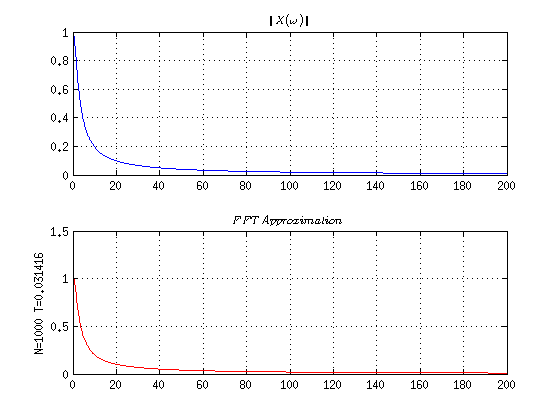
\includegraphics[width=0.8\textwidth]{figs/c4p8.png}
\label{fig:c4p8}
\end{figure} 
